\documentclass{article}

% ready for submission
\usepackage[final]{neurips_2023}

\usepackage[utf8]{inputenc} % allow utf-8 input
\usepackage[T1]{fontenc}    % use 8-bit T1 fonts
\usepackage{hyperref}       % hyperlinks
\usepackage{url}            % simple URL typesetting
\usepackage{booktabs}       % professional-quality tables
\usepackage{amsfonts}       % blackboard math symbols
\usepackage{nicefrac}       % compact symbols for 1/2, etc.
\usepackage{microtype}      % microtypography
\usepackage{xcolor}         % colors
\usepackage{graphicx}       % figures
\graphicspath{{../figures/}} % report figures live in ../figures/

\title{MLPC 2026 Task 4: Data Classification}

\author{%
  Team TEAMNAME \AND
  Author Name 1
  \And
  Author Name 2
}

\begin{document}

\maketitle

% ============================================================
% NOTE: Sections 1 (Dataset Preparation) and 2 (Evaluation) are
% written separately. This file currently contains Sections 3 and 4.
% ============================================================

% \section{Dataset Preparation}  % TODO
% \section{Evaluation}           % TODO

% ============================================================
\section{Experiments}
% ============================================================

We compare two classifiers from different model classes: a linear Support Vector
Machine (one-vs-rest \texttt{LinearSVC}) and CatBoost gradient-boosted trees (one
binary model per class). To keep the comparison fair, both use the identical
collector-level 70/15/15 split (seed 42, so no collector appears in two folds and
recording-style leakage is impossible), the same 480-dimensional mean+std feature
set, per-class decision thresholds tuned on the validation set to maximize F1,
and class weighting to counter the strong imbalance. The SVM additionally z-score
standardizes the features (statistics fit on train only), since linear models are
scale-sensitive whereas trees are not. Hyperparameters and the final model are
selected by \emph{macro}-F1, the metric justified in Section~2 for this
imbalanced multi-label task, and both are compared to the stratified-random
baseline of Section~2.

\textbf{SVM ($C$).} The single most important \texttt{LinearSVC} hyperparameter
is the inverse regularization strength $C$: small $C$ enforces a wider margin
(more bias), large $C$ fits the training data harder (more variance). Validation
macro-F1 (Figure~\ref{fig:svm}) peaks at $C=0.001$ ($0.473$) and is slightly
lower for both stronger ($0.0001$: $0.469$) and weaker ($0.01$: $0.466$)
regularization; an initial wider sweep showed larger $C$ ($\geq0.1$) to be both
worse and disproportionately slower to fit, so we focused on the
strongly-regularized regime. Tuning the per-class thresholds is essential, raising
the SVM from $0.386$ at the default decision boundary to $0.480$ macro-F1.

\begin{figure}[h]
  \centering
  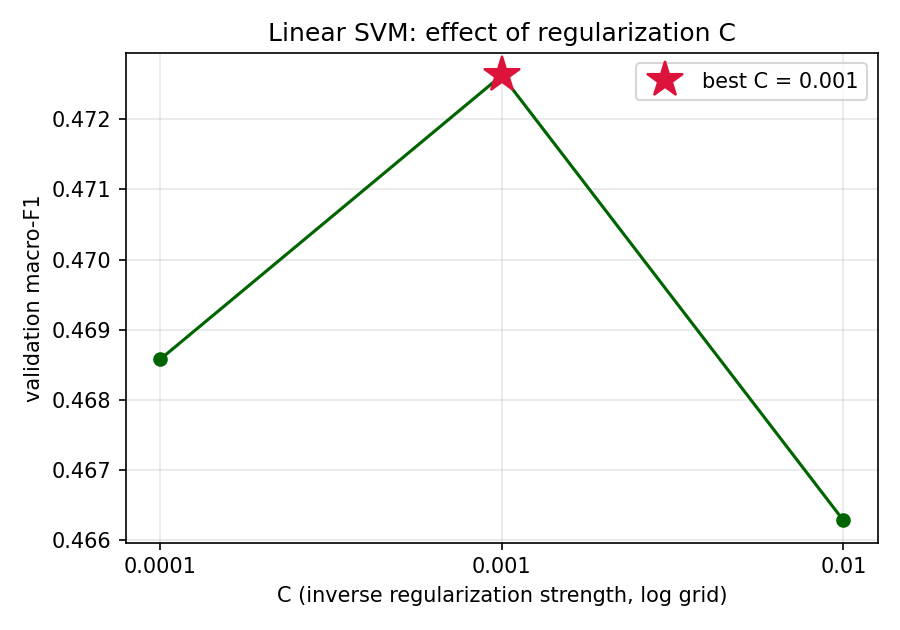
\includegraphics[width=0.5\linewidth]{svm_hyperparams.png}
  \caption{Linear SVM: validation macro-F1 vs.\ regularization $C$ (log grid),
  best at $C=0.001$.}
  \label{fig:svm}
\end{figure}

\textbf{CatBoost (depth, learning rate, L2).} We vary the three most influential
knobs one at a time around the defaults (Figure~\ref{fig:cb}). Tree \emph{depth}
controls interaction order and peaks at $6$ (shallower underfits, deeper
overfits); the \emph{learning rate} is best at $0.1$ ($0.2$ overshoots and
collapses to $0.521$); and a slightly stronger \emph{L2 leaf regularization} of
$6$ beats the default $3$. The curves are otherwise flat (all within
$\approx0.006$ macro-F1), so CatBoost is robust to these settings; we select
\texttt{depth=6, learning\_rate=0.1, l2\_leaf\_reg=6}.

\begin{figure}[h]
  \centering
  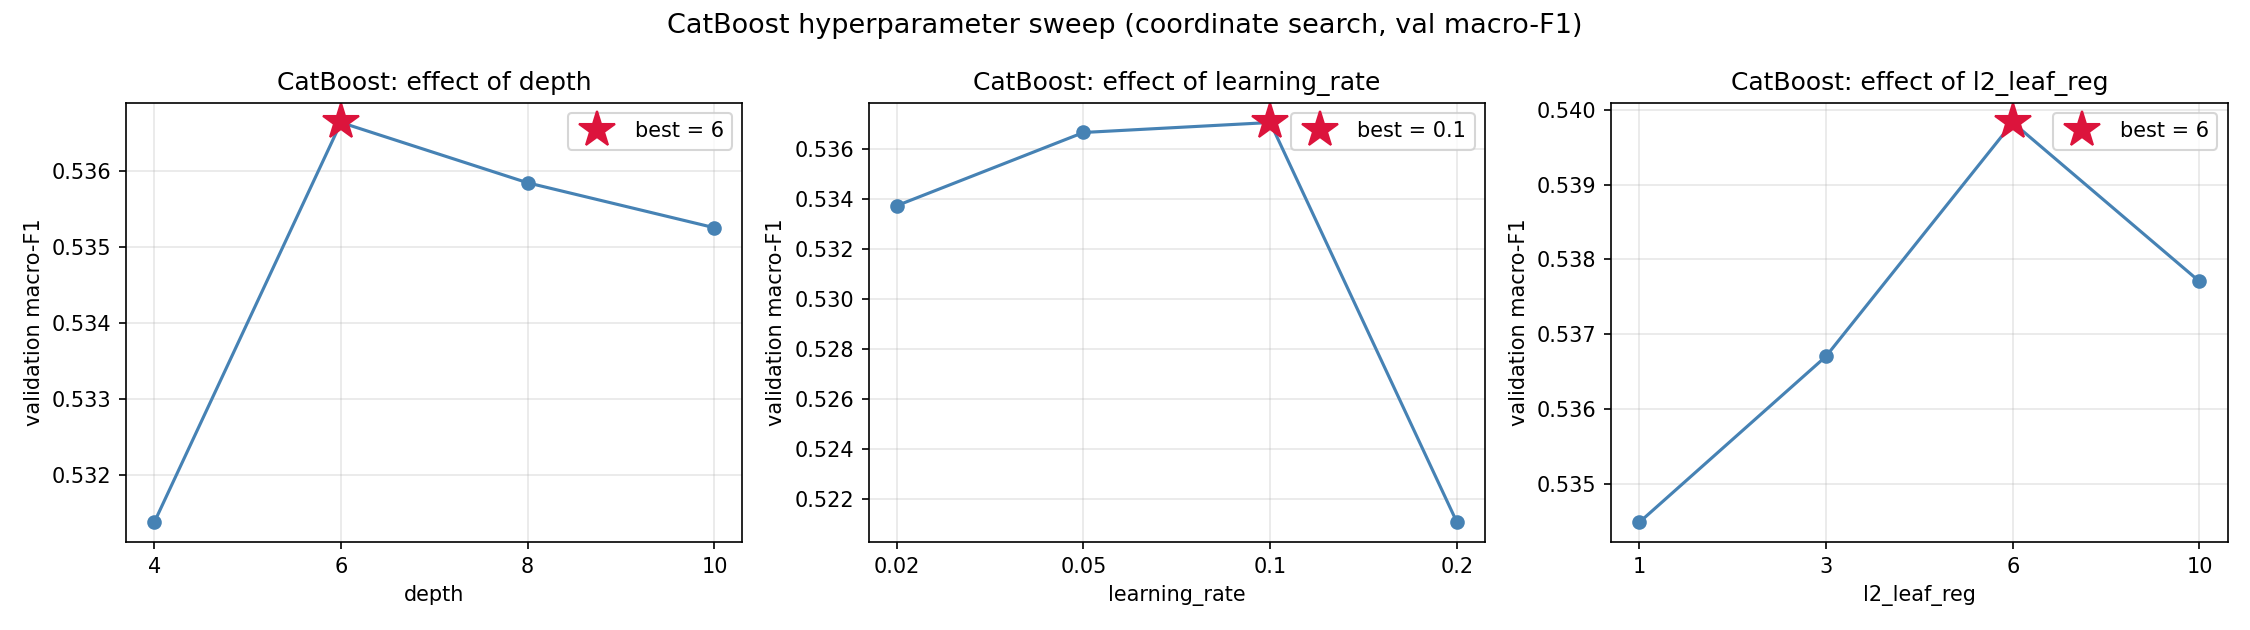
\includegraphics[width=0.92\linewidth]{catboost_hyperparams.png}
  \caption{CatBoost coordinate sweep: validation macro-F1 vs.\ each
  hyperparameter (others held at default). Selected values starred.}
  \label{fig:cb}
\end{figure}

\textbf{Comparison.} Table~\ref{tab:final} reports test performance with the
selected hyperparameters. Both models hugely beat the baseline ($0.063$ macro-F1):
the SVM reaches $0.480$ and CatBoost $0.535$, an $8.5\times$ improvement.
Threshold tuning is the single biggest post-processing gain for both (SVM
$+0.094$, CatBoost $+0.064$). CatBoost is the stronger model by $+0.056$ macro-F1.
The per-class breakdown (Table~\ref{tab:perclass}) explains why: both models agree
on which classes are easy (sustained, spectrally distinctive sources like
\emph{running\_water}, \emph{keyboard\_typing}, \emph{vacuum\_cleaner}) and which
are hard (rare, transient ``open/close'' events like \emph{light\_switch},
\emph{wardrobe}, \emph{window}), so the difficulty is intrinsic to the data rather
than the model. CatBoost's advantage is largest exactly where nonlinear feature
interactions help --- \emph{vacuum\_cleaner} ($+0.12$), \emph{toilet\_flushing}
($+0.11$), \emph{keychain} ($+0.09$) --- which the linear SVM cannot represent.
The only class where the SVM edges ahead is \emph{phone\_ringing}, and
\emph{bell\_ringing} is a tie. CatBoost's practical cost is training one model per
class; the SVM is conceptually simpler but never competitive and slow at large
$C$.

\begin{table}[h]
  \begin{minipage}{0.46\linewidth}
    \centering
    \caption{Test performance (tuned thresholds unless noted); identical split,
    features and baseline.}
    \label{tab:final}
    \begin{tabular}{lcc}
      \toprule
      Model & F1\textsubscript{ma} & F1\textsubscript{mi} \\
      \midrule
      Baseline (random)        & 0.063 & 0.090 \\
      SVM (default thr.)       & 0.386 & 0.416 \\
      SVM (tuned thr.)         & 0.480 & 0.559 \\
      CatBoost (thr.\ 0.5)     & 0.471 & 0.515 \\
      \textbf{CatBoost (tuned)}& \textbf{0.535} & \textbf{0.616} \\
      \bottomrule
    \end{tabular}
  \end{minipage}\hfill
  \begin{minipage}{0.5\linewidth}
    \centering
    \caption{Per-class test F1 (tuned), sorted by CatBoost.}
    \label{tab:perclass}
    \small
    \begin{tabular}{lcc}
      \toprule
      Class & SVM & CatBoost \\
      \midrule
      running\_water    & 0.74 & \textbf{0.77} \\
      keyboard\_typing  & 0.72 & \textbf{0.76} \\
      vacuum\_cleaner   & 0.61 & \textbf{0.73} \\
      cutlery\_dishes   & 0.55 & \textbf{0.63} \\
      microwave         & 0.57 & \textbf{0.61} \\
      phone\_ringing    & \textbf{0.64} & 0.61 \\
      keychain          & 0.51 & \textbf{0.60} \\
      coffee\_machine   & 0.56 & \textbf{0.58} \\
      footsteps         & 0.52 & \textbf{0.58} \\
      toilet\_flushing  & 0.47 & \textbf{0.58} \\
      bell\_ringing     & 0.46 & 0.46 \\
      door\_open\_close & 0.33 & \textbf{0.39} \\
      window\_open\_close & 0.22 & \textbf{0.31} \\
      wardrobe\_drawer  & 0.20 & \textbf{0.26} \\
      light\_switch     & 0.09 & \textbf{0.15} \\
      \bottomrule
    \end{tabular}
  \end{minipage}
\end{table}

% ============================================================
\section{Case Study and Reflection}
% ============================================================

We qualitatively inspect the tuned CatBoost detector on two test recordings
(collectors unseen in training). For each we show a per-segment timeline of the
15 classes over time, overlaying predicted vs.\ expected labels coloured as true
positive (correct detection), false positive (false alarm), false negative
(missed), or true negative.

\textbf{File 002675} (Figure~\ref{fig:cs1}, 43 segments, 6 classes) is a busy
scene. The central \emph{footsteps} block (12.5--17.5\,s) is detected almost
perfectly, but \emph{footsteps} also fires repeatedly in earlier segments where
it is not annotated --- high recall, poor precision for this impulsive, broadband
class. \emph{running\_water} shows the opposite failure: a false alarm at the
start, one correct segment, then a long missed stretch, i.e.\ the detector latches
onto the onset but loses the sustained part. \emph{cutlery\_dishes} (10 segments)
is missed entirely, and \emph{door\_open\_close} is correctly caught near the end.

\textbf{File 000118} (Figure~\ref{fig:cs2}, 34 segments, 5 classes) is dominated
by a vacuum cleaner that is largely missed (15 of 19 segments are false
negatives) despite its strong overall F1 ($0.73$): the model only catches the
loudest central portion, suggesting it keys on intensity rather than a stable
spectral signature, so the quieter onset and tail are lost. \emph{running\_water}
at the start is detected cleanly, while \emph{footsteps} again mixes a correct
block with scattered false alarms.

\begin{figure}[h]
  \centering
  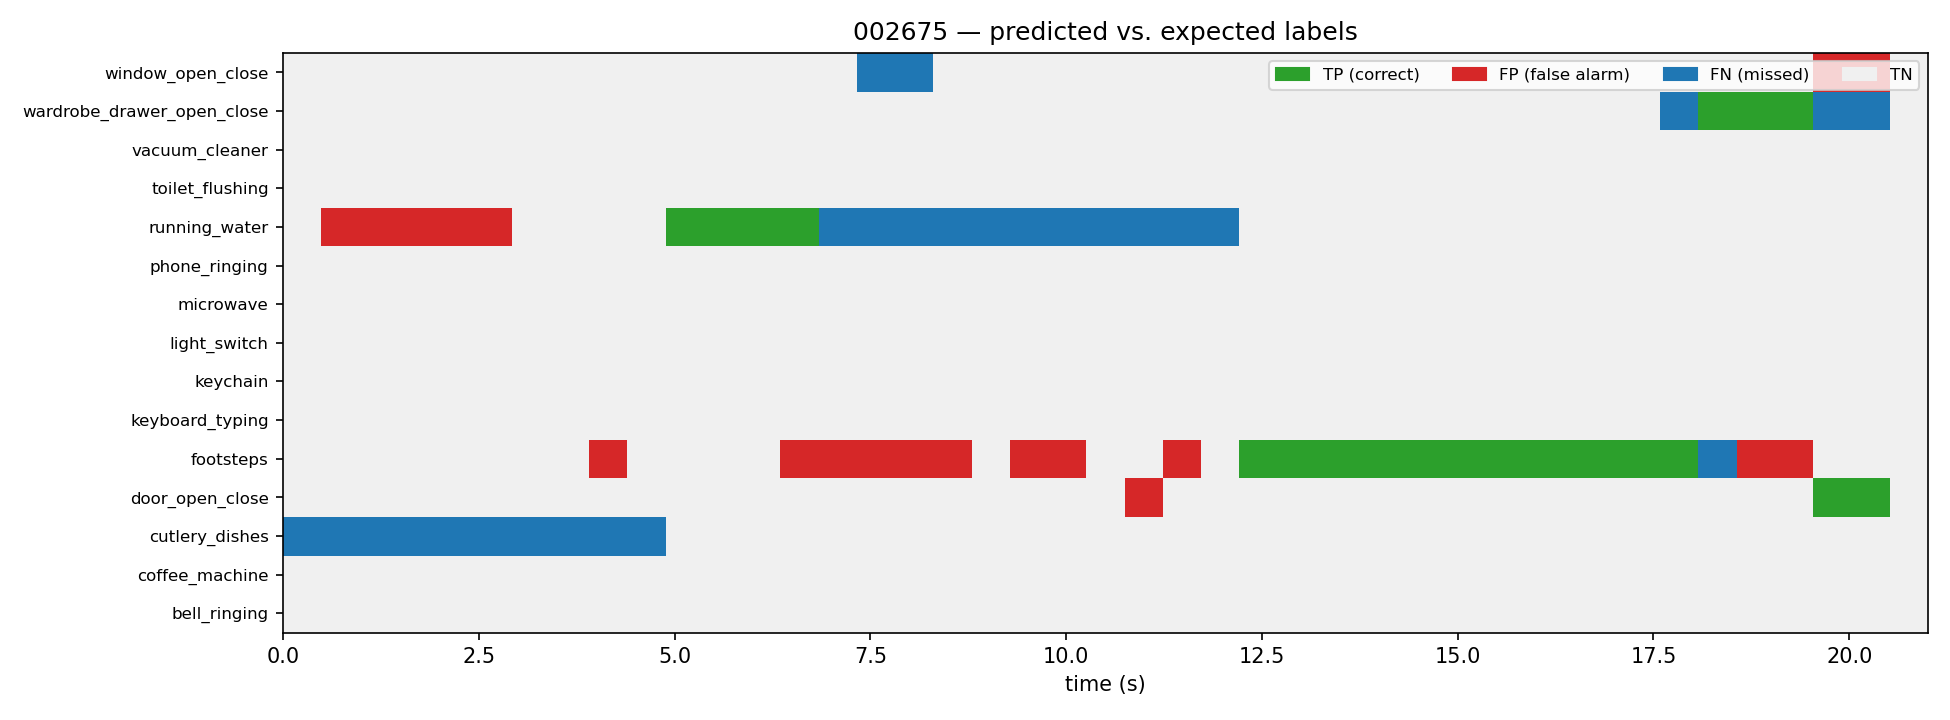
\includegraphics[width=0.85\linewidth]{case_study_002675.png}
  \caption{File 002675 -- predicted vs.\ expected labels per class over time
  (green=correct, red=false alarm, blue=missed, grey=true negative).}
  \label{fig:cs1}
\end{figure}

\textbf{Reflection.} Per-class test F1 ranges from $0.77$ (\emph{running\_water})
to $0.15$ (\emph{light\_switch}). The reliable classes are sustained, spectrally
rich sources; the hardest are rare, brief ``open/close'' events that are both
heavily under-represented and acoustically transient with no characteristic
spectrum. The cross-class confusion matrix (Figure~\ref{fig:cs2}, right) shows the
errors are perceptually plausible rather than random:
\emph{bell}$\leftrightarrow$\emph{phone} (both tonal ringing),
\emph{door}$\leftrightarrow$\emph{window} (near-identical open/close events), and
\emph{cutlery}$\leftrightarrow$\emph{water}/\emph{keychain} (metallic, clattering
kitchen sounds that co-occur). The brightest diagonals match the highest per-class
F1, while the near-empty \emph{light\_switch} row confirms it almost never fires
confidently --- consistent with the imperfect upper bound implied by annotator
disagreement (Section~2). Overall the detector is strong on sustained, distinctive
events and weak on rare impulsive ones, and its mistakes are dominated by
confusions between same-family sounds.

\begin{figure}[h]
  \centering
  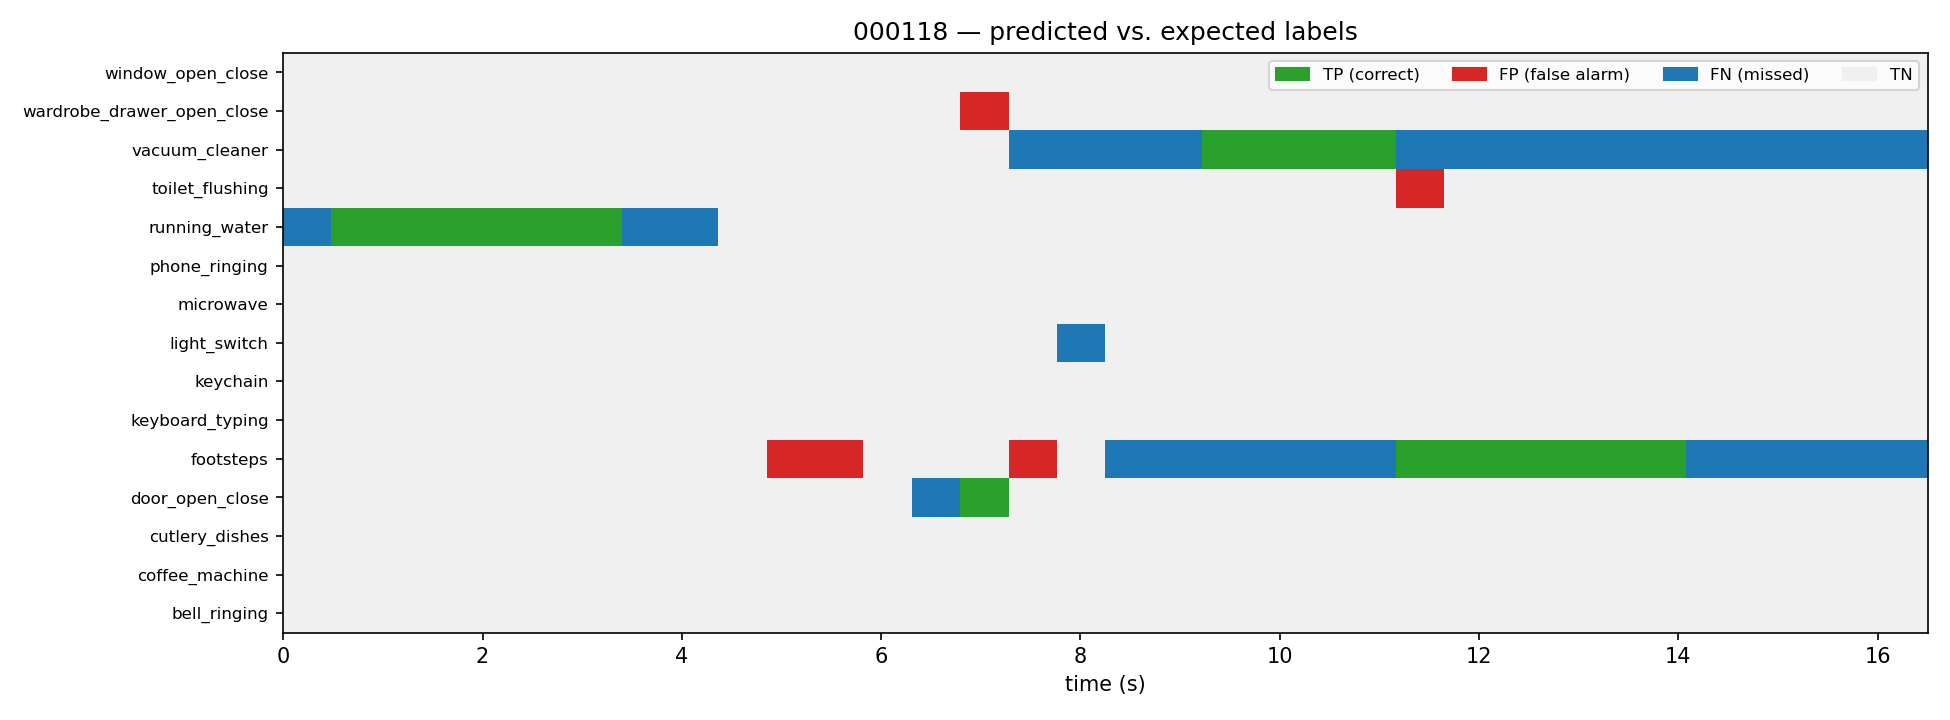
\includegraphics[width=0.6\linewidth]{case_study_000118.png}\hfill
  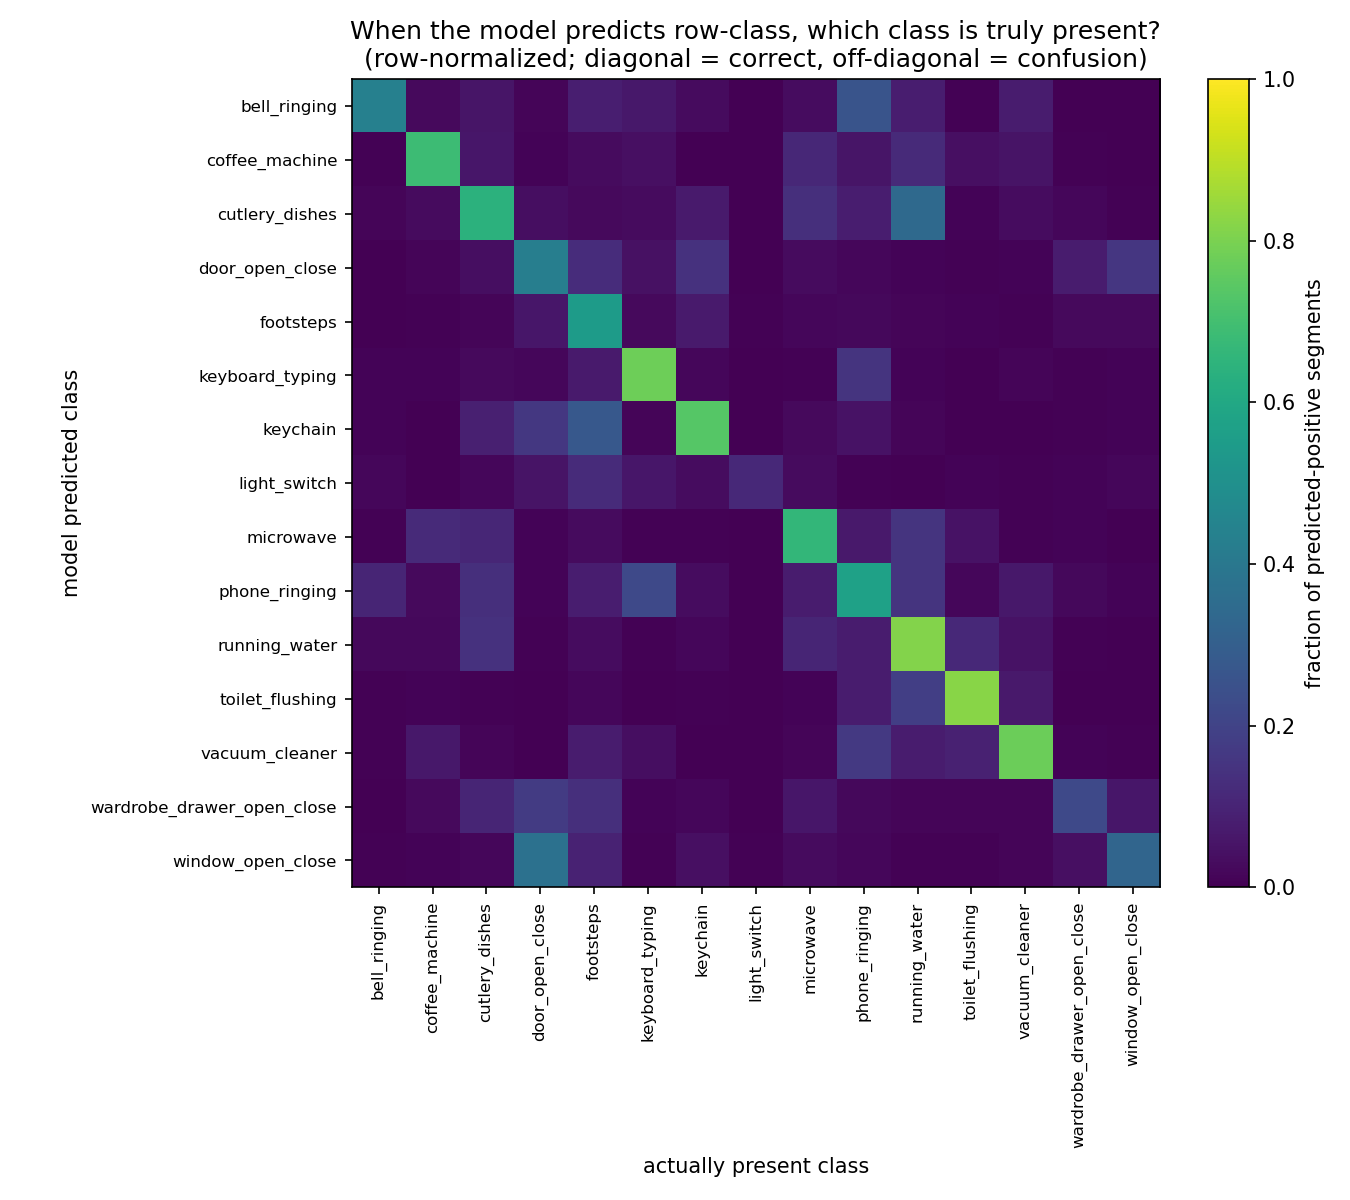
\includegraphics[width=0.38\linewidth]{class_confusion.png}
  \caption{Left: file 000118 -- predicted vs.\ expected labels (same legend as
  Figure~\ref{fig:cs1}); the vacuum cleaner (long blue band) is mostly missed
  outside its loudest portion. Right: cross-class confusion (row-normalized over
  predicted-positive segments); off-diagonal mass marks systematic confusions.}
  \label{fig:cs2}
\end{figure}

% ============================================================
% \section{Disclosure of LLM and AI Tool Use}  % TODO
% ============================================================

\end{document}
